% This is the Reed College LaTeX thesis template. Most of the work
% for the document class was done by Sam Noble (SN), as well as this
% template. Later comments etc. by Ben Salzberg (BTS). Additional
% restructuring and APA support by Jess Youngberg (JY).
% Your comments and suggestions are more than welcome; please email
% them to cus@reed.edu
%
% See https://www.reed.edu/cis/help/LaTeX/index.html for help. There are a
% great bunch of help pages there, with notes on
% getting started, bibtex, etc. Go there and read it if you're not
% already familiar with LaTeX.
%
% Any line that starts with a percent symbol is a comment.
% They won't show up in the document, and are useful for notes
% to yourself and explaining commands.
% Commenting also removes a line from the document;
% very handy for troubleshooting problems. -BTS

% As far as I know, this follows the requirements laid out in
% the 2002-2003 Senior Handbook. Ask a librarian to check the
% document before binding. -SN

%%
%% Preamble
%%
% \documentclass{<something>} must begin each LaTeX document
\documentclass[12pt,twoside]{reedthesis}
% Packages are extensions to the basic LaTeX functions. Whatever you
% want to typeset, there is probably a package out there for it.
% Chemistry (chemtex), screenplays, you name it.
% Check out CTAN to see: https://www.ctan.org/
%%
\usepackage{graphicx,latexsym}
\usepackage{amsmath}
\usepackage{amssymb,amsthm}
\usepackage{longtable,booktabs,setspace}
\usepackage{chemarr} %% Useful for one reaction arrow, useless if you're not a chem major
\usepackage[hyphens]{url}
% Added by CII
\usepackage{hyperref}
\usepackage{lmodern}
\usepackage{float}
\floatplacement{figure}{H}
% Thanks, @Xyv
\usepackage{calc}
% End of CII addition
\usepackage{rotating}

% Next line commented out by CII
%%% \usepackage{natbib}
% Comment out the natbib line above and uncomment the following two lines to use the new
% biblatex-chicago style, for Chicago A. Also make some changes at the end where the
% bibliography is included.
%\usepackage{biblatex-chicago}
%\bibliography{thesis}


% Added by CII (Thanks, Hadley!)
% Use ref for internal links
\renewcommand{\hyperref}[2][???]{\autoref{#1}}
\def\chapterautorefname{Chapter}
\def\sectionautorefname{Section}
\def\subsectionautorefname{Subsection}
% End of CII addition

% Added by CII
\usepackage{caption}
\captionsetup{width=5in}
% End of CII addition

% \usepackage{times} % other fonts are available like times, bookman, charter, palatino

% Syntax highlighting #22

% To pass between YAML and LaTeX the dollar signs are added by CII
\title{Mean temperature, fluctuation magnitude, and level of biological organization affect biological responses amidst thermal variability: a meta-analysis}
\author{Margaret Anne Slein}
% The month and year that you submit your FINAL draft TO THE LIBRARY (May or December)
\date{May 2021}
\division{Mathematical and Natural Sciences}
\advisor{Sam Fey}
\institution{Reed College}
\degree{Bachelor of Arts}
%If you have two advisors for some reason, you can use the following
% Uncommented out by CII
% End of CII addition

%%% Remember to use the correct department!
\department{Biology}
% if you're writing a thesis in an interdisciplinary major,
% uncomment the line below and change the text as appropriate.
% check the Senior Handbook if unsure.
%\thedivisionof{The Established Interdisciplinary Committee for}
% if you want the approval page to say "Approved for the Committee",
% uncomment the next line
%\approvedforthe{Committee}

% Added by CII
%%% Copied from knitr
%% maxwidth is the original width if it's less than linewidth
%% otherwise use linewidth (to make sure the graphics do not exceed the margin)
\makeatletter
\def\maxwidth{ %
  \ifdim\Gin@nat@width>\linewidth
    \linewidth
  \else
    \Gin@nat@width
  \fi
}
\makeatother

% From {rticles}

\renewcommand{\contentsname}{Table of Contents}
% End of CII addition

\setlength{\parskip}{0pt}

% Added by CII

\providecommand{\tightlist}{%
  \setlength{\itemsep}{0pt}\setlength{\parskip}{0pt}}

\Acknowledgements{
The future is bright, the future is dark

Time stands still, yet flies like a lark

Memories endure and memories fade

People are rough, yet smooth like suede

The days seem long, the days seem short

It rains all year, until the sunshine retorts

Reed is an experience, Reed is a place

Reed is a journey of learning how to keep pace

Reed is a individual, Reed is a kollective

Reed is space for being reflective

Reed is the present, Reed is the past

Reed is the net for our future that we cast

To those from Reed

To those from before

To those from the outside

To those at the core

To those I still talk to

To those I talk to no more

To those still here today

To those who now soar

A few words of dear thanks\ldots{}.

Thank you for the laughs, the tears, the screams

Gratitude for the late nights, the dancing, the dreams

Thank you for the walks, the talks, and meals together

Many thanks for the shenanigans I'll cherish forever

Thank you for the compassion, for the coffee and tea

Appreciation for the love, the hate, and learning to be

Thank you for the support, and most ardently, for embracing me
}

\Dedication{

}

\Preface{

}

\Abstract{
Ecosystems and organisms have experienced variation on many temporal scales, including diurnal changes in light availability, seasonal changes in temperature, and decadal changes in weather patterns. Though scientific literature has continued to highlight the importance of ecologically relevant studies for understanding the persistence and dynamics of ecosystems, there has yet to be a quantitative review of how variability impacts biological responses across taxa and scales of biological organization. Here, we present a quantitative meta-analysis of how thermal variability impacts biological responses across multiple taxa, organism sizes, and levels of biological organization. Our results suggest that the range of temperatures an organism experiences is the most important driver of response magnitude, with the interaction of mean temperature and fluctuation range emerging equally as significant predictors in our model of biological responsiveness to temperature variability. Further, our results also suggest that level of biological organization is a less important, though statistically significant, predictor of organismal responses.
}

	\usepackage{setspace}\onehalfspacing
	\usepackage{booktabs}
\usepackage{longtable}
\usepackage{array}
\usepackage{multirow}
\usepackage{wrapfig}
\usepackage{float}
\usepackage{colortbl}
\usepackage{pdflscape}
\usepackage{tabu}
\usepackage{threeparttable}
\usepackage{threeparttablex}
\usepackage[normalem]{ulem}
\usepackage{makecell}
\usepackage{xcolor}
% End of CII addition
%%
%% End Preamble
%%
%
\begin{document}

% Everything below added by CII
  \maketitle

\frontmatter % this stuff will be roman-numbered
\pagestyle{empty} % this removes page numbers from the frontmatter
  \begin{acknowledgements}
    The future is bright, the future is dark
    
    Time stands still, yet flies like a lark
    
    Memories endure and memories fade
    
    People are rough, yet smooth like suede
    
    The days seem long, the days seem short
    
    It rains all year, until the sunshine retorts
    
    Reed is an experience, Reed is a place
    
    Reed is a journey of learning how to keep pace
    
    Reed is a individual, Reed is a kollective
    
    Reed is space for being reflective
    
    Reed is the present, Reed is the past
    
    Reed is the net for our future that we cast
    
    To those from Reed
    
    To those from before
    
    To those from the outside
    
    To those at the core
    
    To those I still talk to
    
    To those I talk to no more
    
    To those still here today
    
    To those who now soar
    
    A few words of dear thanks\ldots{}.
    
    Thank you for the laughs, the tears, the screams
    
    Gratitude for the late nights, the dancing, the dreams
    
    Thank you for the walks, the talks, and meals together
    
    Many thanks for the shenanigans I'll cherish forever
    
    Thank you for the compassion, for the coffee and tea
    
    Appreciation for the love, the hate, and learning to be
    
    Thank you for the support, and most ardently, for embracing me
  \end{acknowledgements}

  \hypersetup{linkcolor=black}
  \setcounter{secnumdepth}{2}
  \setcounter{tocdepth}{2}
  \tableofcontents

  \listoftables

  \listoffigures
  \begin{abstract}
    Ecosystems and organisms have experienced variation on many temporal scales, including diurnal changes in light availability, seasonal changes in temperature, and decadal changes in weather patterns. Though scientific literature has continued to highlight the importance of ecologically relevant studies for understanding the persistence and dynamics of ecosystems, there has yet to be a quantitative review of how variability impacts biological responses across taxa and scales of biological organization. Here, we present a quantitative meta-analysis of how thermal variability impacts biological responses across multiple taxa, organism sizes, and levels of biological organization. Our results suggest that the range of temperatures an organism experiences is the most important driver of response magnitude, with the interaction of mean temperature and fluctuation range emerging equally as significant predictors in our model of biological responsiveness to temperature variability. Further, our results also suggest that level of biological organization is a less important, though statistically significant, predictor of organismal responses.
  \end{abstract}

\mainmatter % here the regular arabic numbering starts
\pagestyle{fancyplain} % turns page numbering back on

\hypertarget{introduction}{%
\chapter*{Introduction}\label{introduction}}
\addcontentsline{toc}{chapter}{Introduction}

Placeholder

\hypertarget{the-historical-significance-of-variability}{%
\section{The historical significance of variability}\label{the-historical-significance-of-variability}}

\hypertarget{relevant-significance-of-variability-today}{%
\section{Relevant significance of variability today}\label{relevant-significance-of-variability-today}}

\hypertarget{why-this-study-on-variability-matters}{%
\section{Why this study on variability matters}\label{why-this-study-on-variability-matters}}

\hypertarget{background}{%
\chapter{Background}\label{background}}

Placeholder

\hypertarget{environmental-variability}{%
\section{Environmental variability}\label{environmental-variability}}

\hypertarget{mean}{%
\subsection{Mean}\label{mean}}

\hypertarget{amplituderange}{%
\subsection{Amplitude/Range}\label{amplituderange}}

\hypertarget{duration}{%
\subsection{Duration}\label{duration}}

\hypertarget{predictability}{%
\subsection{Predictability}\label{predictability}}

\hypertarget{link-between-temporal-and-spatial-variability}{%
\subsection{Link between temporal and spatial variability}\label{link-between-temporal-and-spatial-variability}}

\hypertarget{temperature-variability}{%
\section{Temperature variability}\label{temperature-variability}}

\hypertarget{what-is-temperature-variability}{%
\subsection{What is temperature variability?}\label{what-is-temperature-variability}}

\hypertarget{why-is-temperature-variability-important-to-ecological-processes}{%
\subsection{Why is temperature variability important to ecological processes?}\label{why-is-temperature-variability-important-to-ecological-processes}}

\hypertarget{jensens-inequality-and-its-impacts-on-metabolic-rate}{%
\subsection{Jensen's Inequality and its impacts on metabolic rate}\label{jensens-inequality-and-its-impacts-on-metabolic-rate}}

\hypertarget{relevancy-of-thermal-variability-in-the-modern-context}{%
\subsection{Relevancy of thermal variability in the modern context}\label{relevancy-of-thermal-variability-in-the-modern-context}}

\hypertarget{objectives-driving-questions-hypotheses}{%
\section{Objectives, driving questions, hypotheses}\label{objectives-driving-questions-hypotheses}}

\hypertarget{methods}{%
\chapter{Methods}\label{methods}}

Placeholder

\hypertarget{data-extraction-and-analysis}{%
\section{Data extraction and analysis}\label{data-extraction-and-analysis}}

\hypertarget{metafor}{%
\section{\texorpdfstring{\emph{Metafor}}{Metafor}}\label{metafor}}

\hypertarget{results}{%
\chapter{Results}\label{results}}
\begin{figure}

{\centering 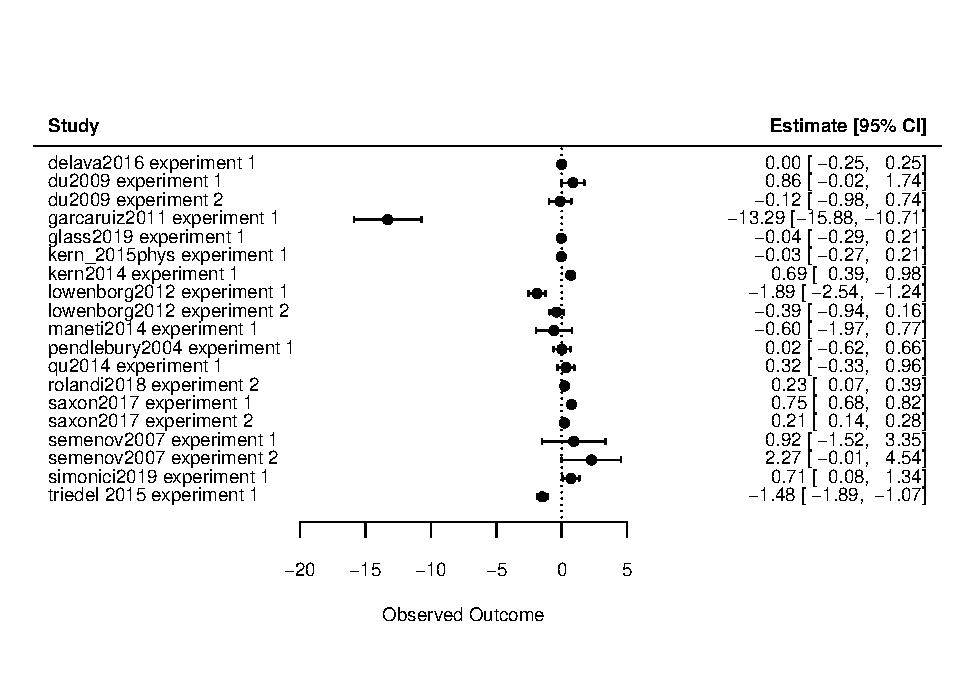
\includegraphics[width=0.95\linewidth]{thesis_files/figure-latex/unnamed-chunk-2-1} 

}

\caption[Forest plot of effect sizes]{Forest plot of effects sizes by study and experiment within a study. Data indicate that both within and across studies, there were a wide range of effect sizes, likely due to experimental design (including fluctuation range, mean temperature, etc.) Each point represents an average of SMD for multiple responses within each experiment in a single study. Accordingly, the error bars represent an average of variance across multiple responses within a single experiment.}\label{fig:unnamed-chunk-2}
\end{figure}
Overall, even our simple model demonstrated that the intercept was not significant but there was significant heterogeneity across studies (n=140, z= 0.79, p \textless{} 0.0001), as demonstrated by Figure 3.1. These results allowed us to reject the null hypothesis that there are no significant differences between SMD across the studies included in analysis (see Appendix Figure 1). This then allowed us to proceed in further detail how different covariates were influencing the effect sizes specifically.

Our full model, including 7 covariates (all covariates in Table 2.2, an additional interaction term between fluctuation range and mean temperature, and excluding thermal stress), responses were still significantly different from each other when accounting for the nested structure of responses, experiments, and studies (QM = 191.3722, df = 7, p \textless{} 0.0001). Further, fluctuation range and the interaction term between fluctuation range and mean temperature were statistically significant in the model (n=140, df = 7, p \textless{} 0.00001). Organization level was also important in the model, as a statistically significant covariate (n=140, df= 7, p \textless{} 0.05).
\begin{figure}

{\centering 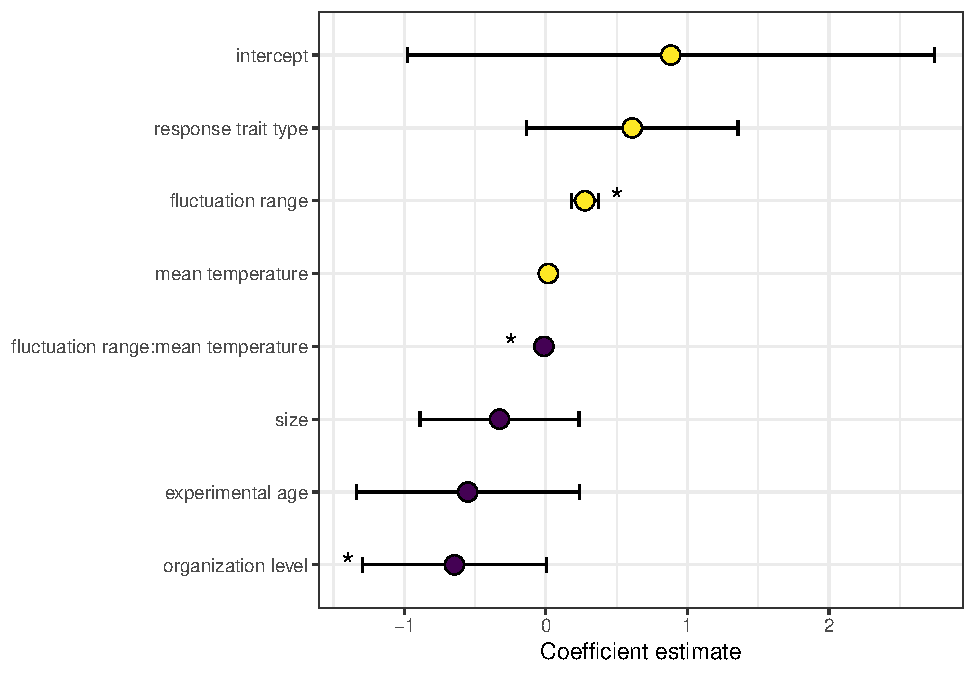
\includegraphics[width=0.95\linewidth]{thesis_files/figure-latex/unnamed-chunk-3-1} 

}

\caption[Coefficient estimates for full model]{Coefficient estimates for each covariate in the full model, where * signify statistically significant model predictors.  Error bars represent 95 percent confidence intervals. Yellow indicates a positive coefficient estimate, purple indicates a negative coefficient estimate.}\label{fig:unnamed-chunk-3}
\end{figure}
\clearpage

Fluctuation range had a positive estimate while the interaction term between range and mean temperature was only slightly negative, both of which were statistically significant (n=140, df=7, p \textless{} 0.001 level (Figure 3.2). The most negative estimate, organization level (n=140), was also significantly influential in our model (n=140, df=7, p \textless{} 0.05).The additional negative estimates of our model coefficients, experimental age and size, were not statistically significant. In our analysis of thermal stress via a separate random effects model, we found thermal stress was not statistically significant (n=132, df=1, p = 0.4855) in explaining the effect size (Table 3.1).
\begin{table}[!h]

\caption[Thermal stress model summary statistics]{\label{tab:unnamed-chunk-4}Model summary statistics for random effects model using thermal stress as sole modifier}
\centering
\begin{tabular}[t]{lrrrrrr}
\toprule
\textbf{Term} & \textbf{estimate} & \textbf{se} & \textbf{zval} & \textbf{pval} & \textbf{ci.lb} & \textbf{ci.ub}\\
\midrule
\cellcolor{gray!6}{intercept} & \cellcolor{gray!6}{0.2050} & \cellcolor{gray!6}{0.1846} & \cellcolor{gray!6}{1.1104} & \cellcolor{gray!6}{0.2668} & \cellcolor{gray!6}{-0.1568} & \cellcolor{gray!6}{0.5669}\\
stressful & -0.0489 & 0.0702 & -0.6975 & 0.4855 & -0.1864 & 0.0886\\
\bottomrule
\end{tabular}
\end{table}
\clearpage

The interaction between fluctuation range and mean temperature as well as effect size is best displayed in Figure 3.3. At lower mean temperatures, higher fluctuation ranges generally have a more positive effect on organism responses and performance, though that trend starkly ends at about \(24^{\circ}\)C. However, at higher mean temperatures, lower fluctuation ranges appear to have an equally positive and negative effect on organism responses and performance (Figure 3.3).
\begin{figure}

{\centering 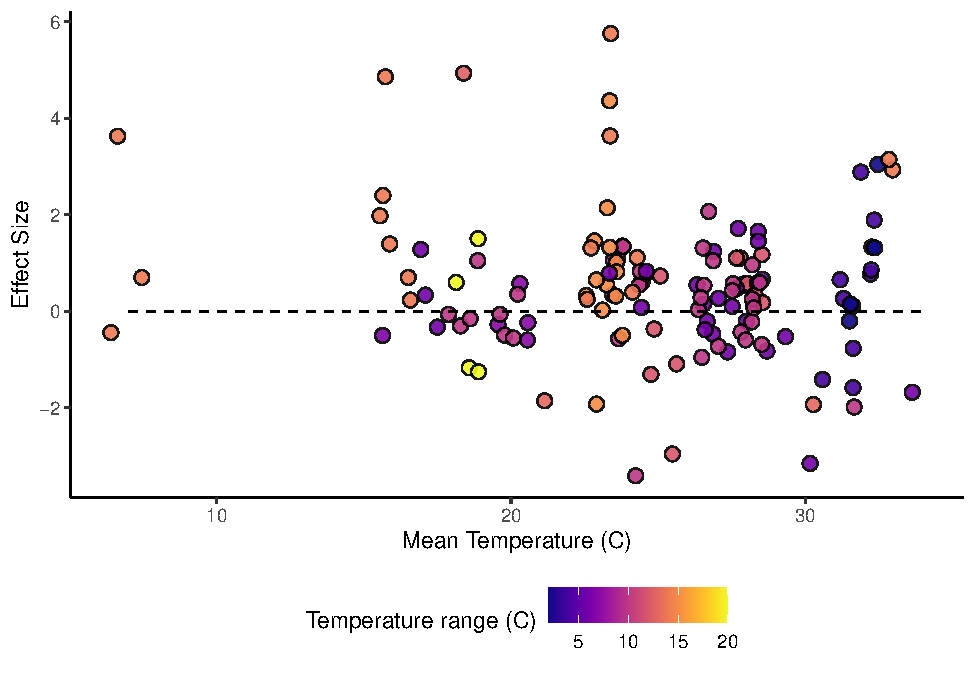
\includegraphics[width=0.9\linewidth]{thesis_files/figure-latex/unnamed-chunk-5-1} 

}

\caption[Scatterplot of relationship between range, mean, and SMD]{Scatterplot describing the relationship between mean temperature, temperature fluctuation range, and SMD. Temperature fluctuation ranged from 0-20°C, mean temperature ranged from 7-33°C. SMD ranged from -4 to 6, restricted based on the distribution of SMD to minimize impact of outliers (see Appendix Figure 2).}\label{fig:unnamed-chunk-5}
\end{figure}
The trend between organization level and temperature fluctuation range, suggests that populations perform better at higher fluctuation ranges than organisms (Figure 3.4). Interestingly, there were not any significant differences between thermal stress (Figure 3.5), life history metric (Figure 3.6), body size (Figure 3.7), or age (Figure 3.8).

When we excluded one highly influential study and included thermal stress in the exclusion model (n=132), size became much more important in the exclusion model (df=8, p \textless{} 0.001) as did mean temperature (df=8, p \textless{} 0.001). Organization level, fluctuation range, and the interaction between fluctuation range and mean temperature became insignificant in the exclusion model (df=8, p \textless{} 0.1).
\begin{figure}

{\centering 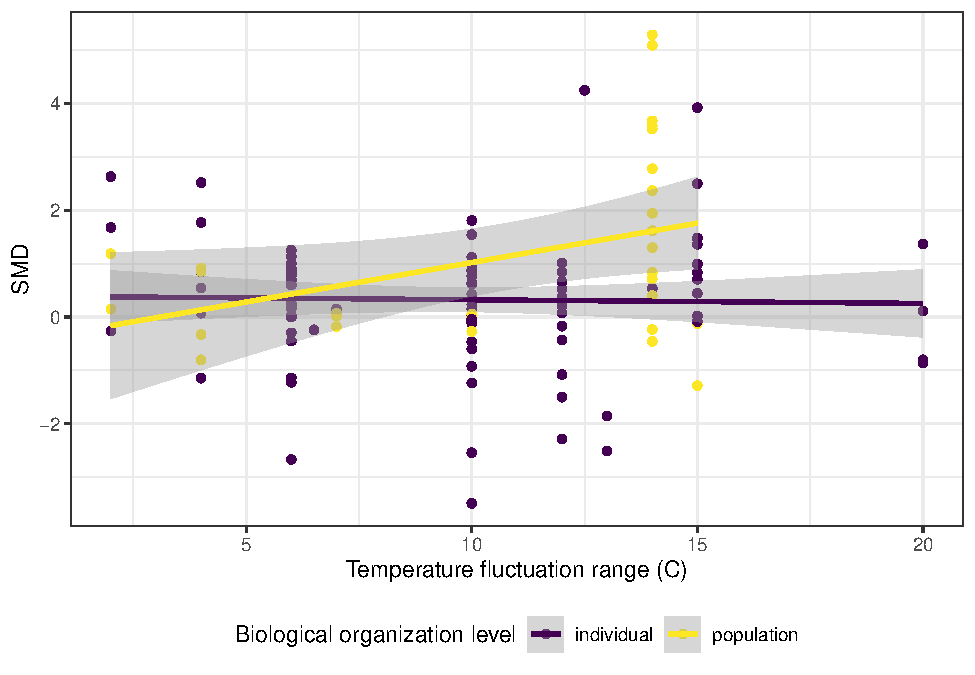
\includegraphics[width=0.85\linewidth]{thesis_files/figure-latex/unnamed-chunk-6-1} 

}

\caption[Effect sizes across temperature range by organization level]{Linear regression of SMD across temperature fluctuation ranges from 0 to 20°C, colored by organization level: individual or population level responses reported in studies.}\label{fig:unnamed-chunk-6}
\end{figure}
\clearpage
\begin{figure}

{\centering 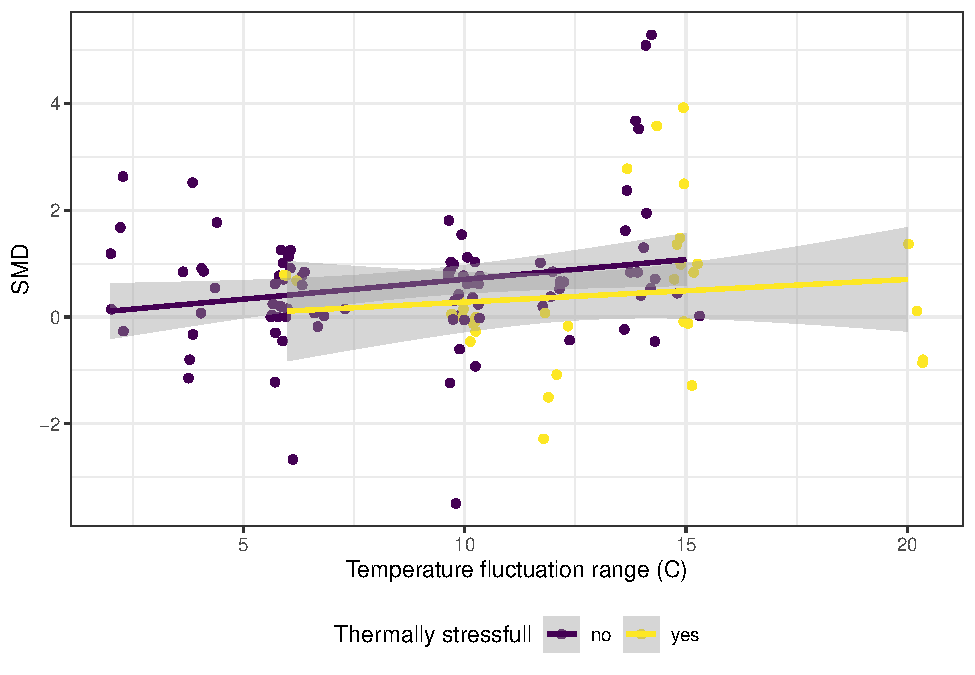
\includegraphics[width=0.85\linewidth]{thesis_files/figure-latex/unnamed-chunk-7-1} 

}

\caption[Effect sizes across temperature range by thermal stress]{Linear regression of SMD across temperature fluctuation ranges from 0 to 20°C, colored by thermal stress.}\label{fig:unnamed-chunk-7}
\end{figure}
\begin{figure}

{\centering 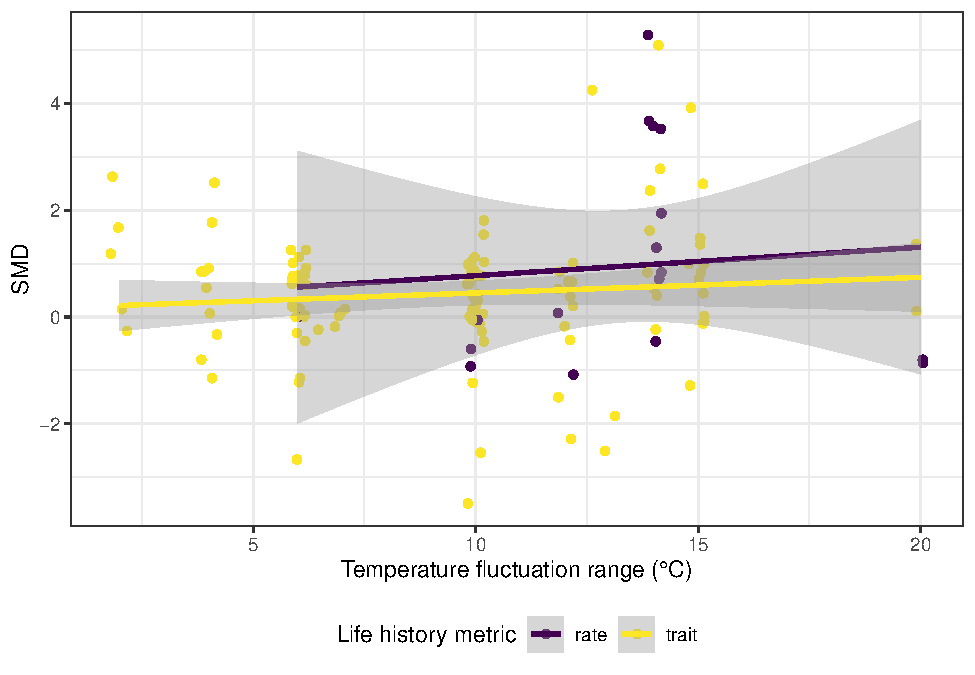
\includegraphics[width=0.85\linewidth]{thesis_files/figure-latex/unnamed-chunk-8-1} 

}

\caption[Effect sizes across temperature range by response type]{Linear regression of SMD across temperature fluctuation ranges from 0 to 20°C, colored by life history metric: responses categorized as rate or trait.}\label{fig:unnamed-chunk-8}
\end{figure}
\begin{figure}

{\centering 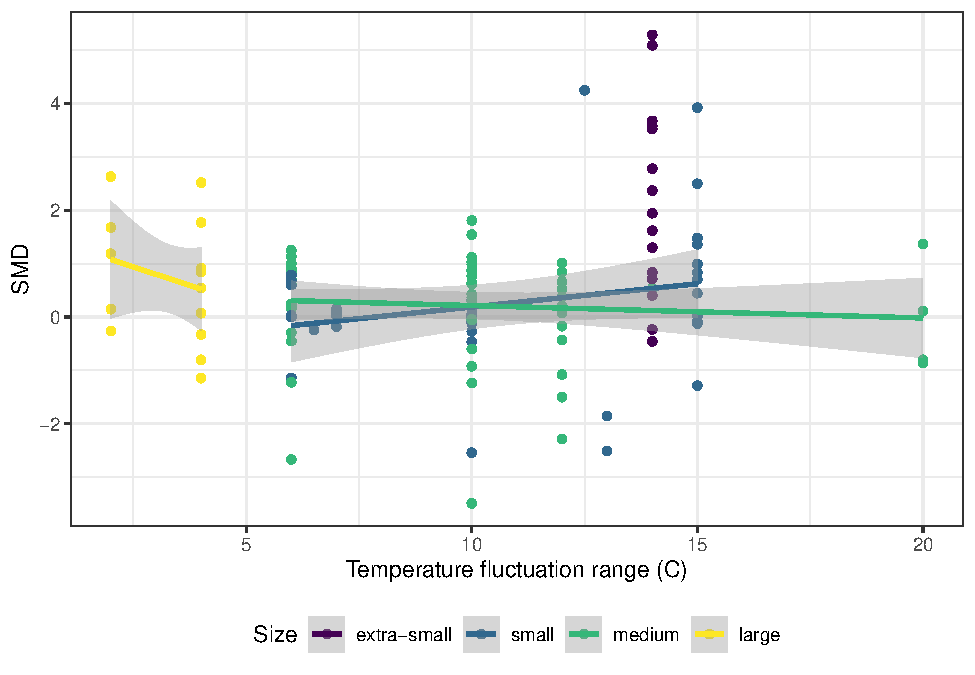
\includegraphics[width=0.85\linewidth]{thesis_files/figure-latex/unnamed-chunk-9-1} 

}

\caption[Effect sizes across temperature range by body size]{Linear regression of SMD across temperature fluctuation ranges from 0 to 20°C, colored by body size: extra-small, small, medium, or large.}\label{fig:unnamed-chunk-9}
\end{figure}
\begin{figure}

{\centering 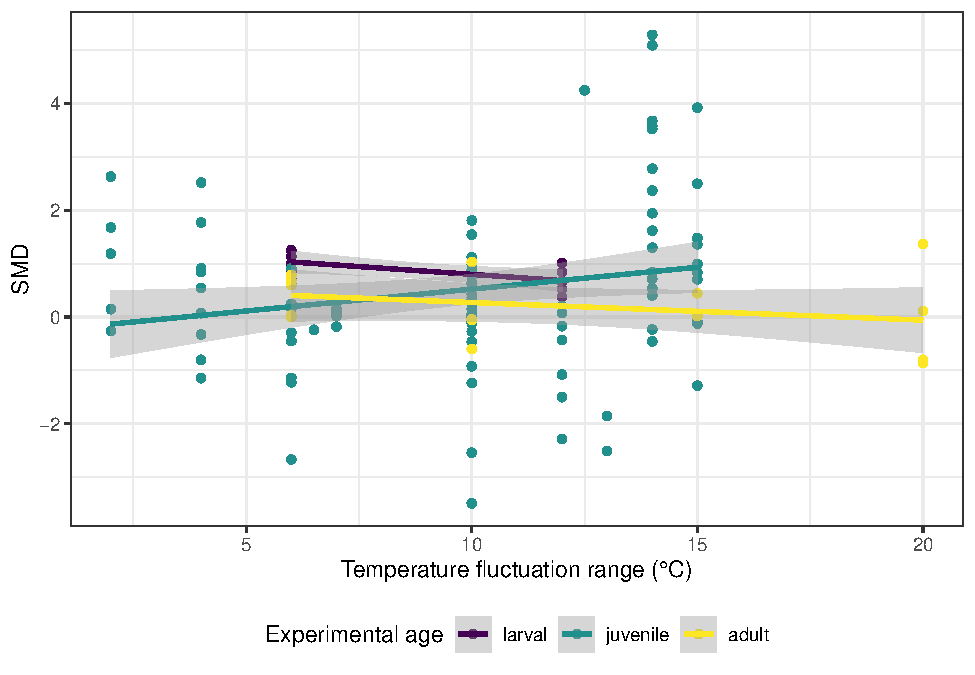
\includegraphics[width=0.85\linewidth]{thesis_files/figure-latex/unnamed-chunk-10-1} 

}

\caption[Effect sizes across temperature range by experimental age]{Linear regression of SMD across temperature fluctuation ranges from 0 to 20°C, colored by experimental age: larval, juvenile, or adult.}\label{fig:unnamed-chunk-10}
\end{figure}
\hypertarget{discussion}{%
\chapter{Discussion}\label{discussion}}

The results of this meta-analysis suggest that fluctuation range is of significant importance to performance, both at the individual and population level. There were not overall differences in the direction of thermally variable environments positively or negatively impacting performance relative to constant environments. However, a considerable amount of variation exists in whether thermally variably environments positively, negatively, or minimally impact performance across studies. Our model results highlight the importance of fluctuation range, mean temperature, and organization level to better understand the variety of effects thermal variation has on organismal responses. These results suggest that mean temperature and fluctuation range must be considered together when understanding the impacts of environmental variability, i.e.~higher fluctuation ranges at lower mean temperatures generally have higher effect sizes compared to higher and lower effects sizes of lower fluctuation ranges at higher mean temperatures. The ways in which organisms, populations, and communities have dealt with natural disturbances has become even more significant in the face of climate change (Sunday, Bates, \& Dulvy, 2012; Vasseur et al., 2014). With global mean temperatures expected to exceed the crucial 2 degree centigrade threshold scientists have deemed ``the point of no return'' (Russill \& Nyssa, 2009), understanding how organisms will cope is key for understanding how ecosystem composition will change at all scales in the next several decades (Cheung, Close, Lam, Watson, \& Pauly, 2008; West, Woodruff, \& Brown, 2002). In this context, perhaps the range of temperatures experienced is of greater importance to predictions of performance under future conditions than simply mean temperature (Vasseur et al., 2014).

These findings underscore the significance of better understanding why differences across studies and experimental designs occurred. Jensen's inequality is one way to conceptualize why responses differ, as averaging nonlinear responses linearly will not accurately predict anticipated performance, in fact, it will underestimate performance (Bernhardt, Sunday, Thompson, \& O'Connor, 2018; Ruel \& Ayres, 1999). The ramifications of underestimating performance and not accounting for environmental variability are inumerable, the biggest of which may be our inability to gauge the critical tipping point for many species' ability to survive. Acclimation may also explain differences in response across studies as the scale on which variation occurs influences how organisms may respond. If organisms' non-genetic phenotypic changes lag behind environmental changes but outpace changes in the constant environment (e.g.~inducing gradual plasticity), acclimation duration may explain mismatches in responses across studies (Kremer, Fey, Arellano, \& Vasseur, 2018). In terms of variability pattern, if an organism experiences environmental variability in uneven intervals, acclimation to previous conditions could explain increases or decreases in performance. Rapid evolution could further explain differences in responses across studies. If organisms are able to keep evolutionary pace with environmental changes via genetic phenotypic changes, responses could be positively affected, as demonstrated in predator-prey system dynamics (Yoshida, Jones, Ellner, Fussmann, \& Hairston, 2003). It is important to note that rapid evolution will only be relevant to population levels responses and not individual level responses.

Equally as interesting as the significant model coefficients were the insignificant model coefficients: body size, thermal stress, life history traits, and experimental age. Body size has been identified as important in the allometric scaling of MTE and it is interesting that in these subsets of studies, body size did not explain the differences in responses across studies. This could simply be because we had a small sample size of studies (n=15). Though multiple responses within each study contributed to a large sample of effect sizes (n=140), there were only a subset of relative body sizes included. It could also provide support for the argument against allometric scaling in MTE, such that there only individualized trends amongst taxonomic groups as opposed to general trends across individuals, populations, and communities of organisms (Clarke, 2006; Clarke \& Johnston, 1999). This theory may also explain why thermal stress was not a significant predictor in our model, if MTE does not aptly describe the patterns that variability in temperature drives.

An important side note is that our full model and thermal stress model differed in the number of studies, as one study, García-Ruiz, Marco, \& Pérez-Moreno (2011), did not have any supplemental information on thermal performance curve points for the taxa used in that study (\emph{Xylotrechus arvicola}). Further, this study happened to contribute highly influential points to our model and subsequent analysis, as our model results change drastically when excluding García-Ruiz et al. (2011) from our full model. We decided to include this study in our analysis because data were extracted from a table, therefore there were no inaccuracies in obtaining the data. It provides an important counter and discussion for how and why responses from different studies may be so different from others.

While body size and thermal stress emerging as not statistically significant coefficients in our model may contradict MTE and its allometric scaling component, an additional analysis, with explicit masses for each of these organisms, would better explore the relationship between thermal variability and MTE. If we were able to obtain additional information about the CTmax, CTmin, thermal breadth, and tolerance range for each of the species included in the analysis, we may also be able to better understand the trends and the significance of variability patterns in dictating responses.

Both the type of response (i.e.~whether it was a rate or trait) and experimental age were also not important predictors in our full model. We expected rates and traits to have different effects, as traits may be more heavily affected by variability because they are not as temporally dynamic as rates. The lack of difference between rates and traits may be because variability is not differentially acting on rate or trait based responses, simply dampening their overall effects. Again, this may be an artifact of having a small sample size, with mainly trait based responses as opposed to rate based responses.

We also expected for experimental age to be an important predictor, as the time period in which an organism experiences thermal variability has been demonstrated to be important for organisms like turtles, relying on TSD for development (Bowden and Paitz 2018). This may again be the result of studies not focused on the larval stage of development, but instead on the juvenile stage. However, there have been meta-analyses, both qualitative (Massey, Holt, Brooks, \& Rollinson, 2019), and quantitative (Noble, Stenhouse, \& Schwanz, 2018), that explicitly looked at the effects of incubation temperature on reptile development, concluding that there is a moderate to large effect of incubation temperature on the magnitude of response (Noble et al., 2018). These results align with patterns of juvenile organisms (e.g.~fish) routinely having higher CTmax values than adults, such that life stage during experimental duration is of importance to thermal tolerance and performance (Moyano et al., 2017; Portner \& Farrell, 2008).

Beyond the data included in our meta-analysis, it is also important to note that there was little variety in the pattern of variation (diurnal, colored noise, etc.) as was initially a question of interest for this project. Diurnal cycles are more correlated than reddened cycles, like seasonal temperatures (Figure 1.3). It is surprising that so many thermal variability studies are focused on diurnal cycles, when in fact, longer-term temperature patterns are more stable than diurnal cycles, and less autocorrelated. Are these diurnal temperature fluctuations accurate for what is expected under natural conditions? This lack of variety in pattern may be due to a lack of consensus on the language used to classify and discuss thermal variability. Though there is a large body of literature that investigates temperature variation, there appears to be dissonance in the scientific literature about the language used to discuss such variation. Many of the background papers pulled from the systematic literature search used temperature variation to mean just different temperatures (Amarasekare \& Savage, 2012) as well as different ranges of temperature, both of which are different concepts. For instance, Amarasekare \& Savage (2012) addressed the need for more complexity when we think about the processes underlying temperature dependent fitness, as fitness is an amalgamation of interactions between different life-history traits. Though temperature variation appeared in the keywords of the article, there was little to no mention of actual thermal variation or variation pattern. Additionally, a subsection of the papers included in our search specifically defined thermal variability as short term changes in temperature, though these studies were mainly focused on explicitly ecologically irrelevant thermal regimes (Colinet, Rinehart, Yocum, \& Greenlee, 2018; Colinet, Sinclair, Vernon, \& Renault, 2015). Using standardized language to describe specific patterns or durations of variability may be helpful in better summarizing the results and conclusions from previous studies.

Many of these studies failed to justify why certain temperatures were chosen as mean temperatures as well as the range of temperatures studied. In order to compile information on the thermal stress of each of the organisms included in the studies of this meta-analysis, additional resources were needed (see Appendix Table 1). Understanding where these organisms' performance falls in relation to temperature on its TPC is crucial for drawing reliable conclusions of how thermal variability affects performance. Without it, only broad conclusions can be drawn, as have been drawn here, that variability and range affects thermal performance.

Several studies made little to no mention of generation time with respect to duration of their experiments or study organisms used. How organisms' life cycles and life spans interact with and are impacted by fluctuation patterns is important for understanding the layers variation permeates and how organisms respond (Bernhardt, O'Connor, Sunday, \& Gonzalez, 2020). This is also pertinent to the scale at which we study variability, given the overrepresentation of diurnal fluctuation patterns featured in our meta-analysis. Diurnal thermal fluctuations may affect organisms with shorter generation times differentially compared to organisms with longer generation times. The converse is true for seasonal or decadal thermal fluctuations.

The results of this analysis differ from previous attempts to understand variability as they quantitatively address how variability affects organisms across taxa, not simply one group. Understanding how allometric scaling and thermal variability patterns interact is important for predicting realistic organismal responses in the face of variable conditions in the environment.

\hypertarget{conclusions-and-future-directions}{%
\chapter*{Conclusions and Future Directions}\label{conclusions-and-future-directions}}
\addcontentsline{toc}{chapter}{Conclusions and Future Directions}

While there are limitations to the reach of this meta-analysis and its results, it is the first cross-taxa quantitative summary of how environmental variability has been studied in the literature. Our results suggest that thermal variability influences responses across several studies, positively as lower mean temperatures with higher fluctuation ranges, and less so at high mean temperatures with lower fluctuation ranges.

However, most importantly, our results highlight the importance of learning from previous research to push how environmental variability is studied further. It has been noted for years the importance of including thermal variability in ecological research, yet there are still an overwhelming number of studies that employ the same patterns of variability with the same lack of reference to thermal performance. Going forward, experiments that explicitly account for and justify variation patterns with respect to generation time, organization level, duration, and relevance to natural conditions are needed. In order to draw conclusions that are relevant to natural conditions, patterns of variability across colors of noise (red, white, etc.) and across lengths of time must be investigated. A larger sample size of studies to draw more robust conclusions with respect to support for or against allometric scaling and MTE with respect to thermal variability would be useful. There is more to be studied on how additional experimental designs, e.g.~acclimation or heat-wave simulations, as well as how biological performance responds to environmental variability. However, this is an important first step in quantitatively summarizing progress so far.

\hypertarget{appendix}{%
\chapter*{Appendix}\label{appendix}}
\addcontentsline{toc}{chapter}{Appendix}

Placeholder

\hypertarget{references}{%
\chapter*{References}\label{references}}
\addcontentsline{toc}{chapter}{References}

Placeholder

\hypertarget{refs}{}
\leavevmode\hypertarget{ref-alagawany_heat_2017}{}%
Alagawany, M., Farag, M., Abd El-Hack, M., \& Patra, A. (2017). Heat stress: Effects on productive and reproductive performance of quail. \emph{World's Poultry Science Journal}, \emph{73}(4), 747--756. \url{http://doi.org/10.1017/S0043933917000782}

\leavevmode\hypertarget{ref-amarasekare_framework_2012}{}%
Amarasekare, P., \& Savage, V. (2012). A framework for elucidating the temperature dependence of fitness. \emph{The American Naturalist}, \emph{179}(2), 178--191. \url{http://doi.org/10.1086/663677}

\leavevmode\hypertarget{ref-baojun_seasonal_2014}{}%
Baojun, S., Wenqi, T., Zhigao, Z., \& Weiguo, D. (2014). The seasonal acclimatisation of locomotion in a terrestrial reptile, plestiodon chinensis(Scincidae). \emph{Asian Herpetological Research}, \emph{5}(3), 197. \url{http://doi.org/10.3724/SP.J.1245.2014.00197}

\leavevmode\hypertarget{ref-bernhardt_life_2020}{}%
Bernhardt, J. R., O'Connor, M. I., Sunday, J. M., \& Gonzalez, A. (2020). Life in fluctuating environments. \emph{Phil. Trans. R. Soc. B}, \emph{375}(1814), 20190454. \url{http://doi.org/10.1098/rstb.2019.0454}

\leavevmode\hypertarget{ref-bernhardt_nonlinear_2018}{}%
Bernhardt, J. R., Sunday, J. M., Thompson, P. L., \& O'Connor, M. I. (2018). Nonlinear averaging of thermal experience predicts population growth rates in a thermally variable environment, 10.

\leavevmode\hypertarget{ref-bronikowski_evolutionary_2001}{}%
Bronikowski, A. M., Bennett, A. F., \& Lenski, R. E. (2001). EVOLUTIONARY ADAPTATION TO TEMPERATURE. VIII. EFFECTS OF TEMPERATURE ON GROWTH RATE IN NATURAL ISOLATES OF ESCHERICHIA COLI AND SALMONELLA ENTERICA FROM DIFFERENT THERMAL ENVIRONMENTS. \emph{Evolution}, \emph{55}(1), 33--40. \url{http://doi.org/10.1111/j.0014-3820.2001.tb01270.x}

\leavevmode\hypertarget{ref-cheung_application_2008}{}%
Cheung, W., Close, C., Lam, V., Watson, R., \& Pauly, D. (2008). Application of macroecological theory to predict effects of climate change on global fisheries potential. \emph{Mar. Ecol. Prog. Ser.}, \emph{365}, 187--197. \url{http://doi.org/10.3354/meps07414}

\leavevmode\hypertarget{ref-clarke_temperature_2006}{}%
Clarke, A. (2006). Temperature and the metabolic theory of ecology. \emph{Funct Ecology}, \emph{20}(2), 405--412. \url{http://doi.org/10.1111/j.1365-2435.2006.01109.x}

\leavevmode\hypertarget{ref-clarke_scaling_1999}{}%
Clarke, A., \& Johnston, N. M. (1999). Scaling of metabolic rate with body mass and temperature in teleost fish. \emph{J Anim Ecology}, \emph{68}(5), 893--905. \url{http://doi.org/10.1046/j.1365-2656.1999.00337.x}

\leavevmode\hypertarget{ref-colinet_mechanisms_2018}{}%
Colinet, H., Rinehart, J. P., Yocum, G. D., \& Greenlee, K. J. (2018). Mechanisms underpinning the beneficial effects of fluctuating thermal regimes in insect cold tolerance. \emph{J Exp Biol}, \emph{221}(14), jeb164806. \url{http://doi.org/10.1242/jeb.164806}

\leavevmode\hypertarget{ref-colinet_insects_2015}{}%
Colinet, H., Sinclair, B. J., Vernon, P., \& Renault, D. (2015). Insects in fluctuating thermal environments. \emph{Annu. Rev. Entomol.}, \emph{60}(1), 123--140. \url{http://doi.org/10.1146/annurev-ento-010814-021017}

\leavevmode\hypertarget{ref-dang_thermal_2019}{}%
Dang, W., Hu, Y.-C., Geng, J., Wang, J., \& Lu, H.-L. (2019). Thermal physiological performance of two freshwater turtles acclimated to different temperatures. \emph{J Comp Physiol B}, \emph{189}(1), 121--130. \url{http://doi.org/10.1007/s00360-018-1194-x}

\leavevmode\hypertarget{ref-delava_effects_2016}{}%
Delava, E., Fleury, F., \& Gibert, P. (2016). Effects of daily fluctuating temperatures on the drosophila--leptopilina boulardi parasitoid association. \emph{Journal of Thermal Biology}, \emph{60}, 95--102. \url{http://doi.org/10.1016/j.jtherbio.2016.06.012}

\leavevmode\hypertarget{ref-doyle_survival_1984}{}%
Doyle, M. P., \& Schoeni, J. L. (1984). Survival and growth characteristics of escherichia coli associated with hemorrhagic colitis. \emph{Applied and Environmental Microbiology}, \emph{48}(4), 855--856. \url{http://doi.org/10.1128/AEM.48.4.855-856.1984}

\leavevmode\hypertarget{ref-du_embryonic_2009}{}%
Du, W.-G., Shen, J.-W., \& Wang, L. (2009). Embryonic development rate and hatchling phenotypes in the chinese three-keeled pond turtle (chinemys reevesii): The influence of fluctuating temperature versus constant temperature. \emph{Journal of Thermal Biology}, \emph{34}(5), 250--255. \url{http://doi.org/10.1016/j.jtherbio.2009.03.002}

\leavevmode\hypertarget{ref-fresquet_response_2011}{}%
Fresquet, N., \& Lazzari, C. R. (2011). Response to heat in rhodnius prolixus: The role of the thermal background. \emph{Journal of Insect Physiology}, \emph{57}(10), 1446--1449. \url{http://doi.org/10.1016/j.jinsphys.2011.07.012}

\leavevmode\hypertarget{ref-garcia-ruiz_effects_2011}{}%
García-Ruiz, E., Marco, V., \& Pérez-Moreno, I. (2011). Effects of variable and constant temperatures on the embryonic development and survival of a new grape pest, xylotrechus arvicola (coleoptera: Cerambycidae). \emph{Environ Entomol}, \emph{40}(4), 939--947. \url{http://doi.org/10.1603/EN11080}

\leavevmode\hypertarget{ref-glass_should_2019}{}%
Glass, J. R., \& Stahlschmidt, Z. R. (2019). Should i stay or should i go? Complex environments influence the developmental plasticity of flight capacity and flight-related trade-offs. \emph{Biological Journal of the Linnean Society}, \emph{128}(1), 59--69. \url{http://doi.org/10.1093/biolinnean/blz073}

\leavevmode\hypertarget{ref-isaac_isaac_2003pdf_2003}{}%
Isaac, L. A. (2003). Isaac\_2003.pdf. University of Victoria. Retrieved from \url{https://dspace.library.uvic.ca/handle/1828/356}

\leavevmode\hypertarget{ref-kern_temperature_2014}{}%
Kern, P., Cramp, R. L., \& Franklin, C. E. (2014). Temperature and UV-b-insensitive performance in tadpoles of the ornate burrowing frog: An ephemeral pond specialist. \emph{Journal of Experimental Biology}, \emph{217}(8), 1246--1252. \url{http://doi.org/10.1242/jeb.097006}

\leavevmode\hypertarget{ref-kern_physiological_2015-3}{}%
Kern, P., Cramp, R. L., \& Franklin, C. E. (2015). Physiological responses of ectotherms to daily temperature variation. \emph{Journal of Experimental Biology}, \emph{218}(19), 3068--3076. \url{http://doi.org/10.1242/jeb.123166}

\leavevmode\hypertarget{ref-khelifa_usefulness_2019}{}%
Khelifa, R., Blanckenhorn, W. U., Roy, J., Rohner, P. T., \& Mahdjoub, H. (2019). Usefulness and limitations of thermal performance curves in predicting ectotherm development under climatic variability. \emph{J Anim Ecol}, \emph{88}(12), 1901--1912. \url{http://doi.org/10.1111/1365-2656.13077}

\leavevmode\hypertarget{ref-klepsatel_variation_2013}{}%
Klepsatel, P., Gáliková, M., De Maio, N., Huber, C. D., Schlötterer, C., \& Flatt, T. (2013). VARIATION IN THERMAL PERFORMANCE AND REACTION NORMS AMONG POPULATIONS OF \emph{DROSOPHILA MELANOGASTER}: THERMAL PERFORMANCE IN DROSOPHILA. \emph{Evolution}, \emph{67}(12), 3573--3587. \url{http://doi.org/10.1111/evo.12221}

\leavevmode\hypertarget{ref-kremer_gradual_2018}{}%
Kremer, C. T., Fey, S. B., Arellano, A. A., \& Vasseur, D. A. (2018). Gradual plasticity alters population dynamics in variable environments: Thermal acclimation in the green alga \emph{chlamydomonas reinhartdii}. \emph{Proc. R. Soc. B.}, \emph{285}(1870), 20171942. \url{http://doi.org/10.1098/rspb.2017.1942}

\leavevmode\hypertarget{ref-krenek_coping_2012}{}%
Krenek, S., Petzoldt, T., \& Berendonk, T. U. (2012). Coping with temperature at the warm edge -- patterns of thermal adaptation in the microbial eukaryote paramecium caudatum. \emph{PLoS ONE}, \emph{7}(3), e30598. \url{http://doi.org/10.1371/journal.pone.0030598}

\leavevmode\hypertarget{ref-lowenborg_how_2012}{}%
Löwenborg, K., Gotthard, K., \& Hagman, M. (2012). How a thermal dichotomy in nesting environments influences offspring of the world's most northerly oviparous snake, \emph{natrix natrix} (colubridae): Grass snake nest-site dichotomy. \emph{Biol J Linn Soc Lond}, \emph{107}(4), 833--844. \url{http://doi.org/10.1111/j.1095-8312.2012.01972.x}

\leavevmode\hypertarget{ref-manenti_predictability_2014-2}{}%
Manenti, T., Sørensen, J. G., Moghadam, N. N., \& Loeschcke, V. (2014). Predictability rather than amplitude of temperature fluctuations determines stress resistance in a natural population of \emph{drosophila simulans}. \emph{J. Evol. Biol.}, \emph{27}(10), 2113--2122. \url{http://doi.org/10.1111/jeb.12463}

\leavevmode\hypertarget{ref-massey_measurement_2019}{}%
Massey, M. D., Holt, S. M., Brooks, R. J., \& Rollinson, N. (2019). Measurement and modelling of primary sex ratios for species with temperature-dependent sex determination. \emph{J Exp Biol}, \emph{222}(1), jeb190215. \url{http://doi.org/10.1242/jeb.190215}

\leavevmode\hypertarget{ref-moyano_effects_2017}{}%
Moyano, M., Candebat, C., Ruhbaum, Y., Álvarez-Fernández, S., Claireaux, G., Zambonino-Infante, J.-L., \& Peck, M. A. (2017). Effects of warming rate, acclimation temperature and ontogeny on the critical thermal maximum of temperate marine fish larvae. \emph{PLoS ONE}, \emph{12}(7), e0179928. \url{http://doi.org/10.1371/journal.pone.0179928}

\leavevmode\hypertarget{ref-noble_developmental_2018}{}%
Noble, D. W. A., Stenhouse, V., \& Schwanz, L. E. (2018). Developmental temperatures and phenotypic plasticity in reptiles: A systematic review and meta-analysis: Incubation temperature and plasticity. \emph{Biol Rev}, \emph{93}(1), 72--97. \url{http://doi.org/10.1111/brv.12333}

\leavevmode\hypertarget{ref-parachu_marco_new_2017}{}%
Parachu Marco, M. V., Leiva, P., Iungman, J. L., Simonici, M. S., \& Pina, C. I. (2017). New evidence characterizing temperature-dependent sex determination in broad-snouted caiman, caiman latirostris. \emph{Herpetological Conservation and Biology}, (12), 78--84.

\leavevmode\hypertarget{ref-pendlebury_variation_2004-1}{}%
Pendlebury, C. J. (2004). Variation in temperature increases the cost of living in birds. \emph{Journal of Experimental Biology}, \emph{207}(12), 2065--2070. \url{http://doi.org/10.1242/jeb.00999}

\leavevmode\hypertarget{ref-pina_effect_2003}{}%
Piña, C. I., Larriera, A., \& Cabrera, M. R. (2003). Effect of incubation temperature on incubation period, sex ratio, hatching success, and survivorship in caiman latirostris (crocodylia, alligatoridae). \emph{Journal of Herpetology}, \emph{37}(1), 199--202. \href{http://doi.org/10.1670/0022-1511(2003)037\%5B0199:EOITOI\%5D2.0.CO;2}{http://doi.org/10.1670/0022-1511(2003)037{[}0199:EOITOI{]}2.0.CO;2}

\leavevmode\hypertarget{ref-portner_ecology_2008}{}%
Portner, H. O., \& Farrell, A. P. (2008). ECOLOGY: Physiology and climate change. \emph{Science}, \emph{322}(5902), 690--692. \url{http://doi.org/10.1126/science.1163156}

\leavevmode\hypertarget{ref-qu_incubation_2014}{}%
Qu, Y.-F., Lu, H.-L., Li, H., \& Ji, X. (2014). Incubation temperature fluctuation does not affect incubation length and hatchling phenotype in the chinese skink plestiodon chinensis. \emph{Journal of Thermal Biology}, \emph{46}, 10--15. \url{http://doi.org/10.1016/j.jtherbio.2014.09.008}

\leavevmode\hypertarget{ref-rolandi_costs_2018}{}%
Rolandi, C., \& Schilman, P. E. (2018). The costs of living in a thermal fluctuating environment for the tropical haematophagous bug, rhodnius prolixus. \emph{Journal of Thermal Biology}, \emph{74}, 92--99. \url{http://doi.org/10.1016/j.jtherbio.2018.03.022}

\leavevmode\hypertarget{ref-ruel_jensens_1999}{}%
Ruel, J. J., \& Ayres, M. P. (1999). Jensen's inequality predicts effects of environmental variation. \emph{Trends in Ecology \& Evolution}, \emph{14}(9), 361--366. \url{http://doi.org/10.1016/S0169-5347(99)01664-X}

\leavevmode\hypertarget{ref-russill_tipping_2009}{}%
Russill, C., \& Nyssa, Z. (2009). The tipping point trend in climate change communication. \emph{Global Environmental Change}, \emph{19}(3), 336--344. \url{http://doi.org/10.1016/j.gloenvcha.2009.04.001}

\leavevmode\hypertarget{ref-saxon_temperature_2018-1}{}%
Saxon, A. D., O'Brien, E. K., \& Bridle, J. R. (2018). Temperature fluctuations during development reduce male fitness and may limit adaptive potential in tropical rainforest \emph{drosophila}. \emph{J. Evol. Biol.}, \emph{31}(3), 405--415. \url{http://doi.org/10.1111/jeb.13231}

\leavevmode\hypertarget{ref-seebacher_embryonic_2014}{}%
Seebacher, F., \& Grigaltchik, V. S. (2014). Embryonic developmental temperatures modulate thermal acclimation of performance curves in tadpoles of the frog limnodynastes peronii. \emph{PLoS ONE}, \emph{9}(9), e106492. \url{http://doi.org/10.1371/journal.pone.0106492}

\leavevmode\hypertarget{ref-semenov_influence_2007}{}%
Semenov, A. V., Van Bruggen, A. H., Van Overbeek, L., Termorshuizen, A. J., \& Semenov, A. M. (2007). Influence of temperature fluctuations on escherichia coli o157:H7 and salmonella enterica serovar typhimurium in cow manure: Effect of temperature fluctuation on human pathogens. \emph{FEMS Microbiology Ecology}, \emph{60}(3), 419--428. \url{http://doi.org/10.1111/j.1574-6941.2007.00306.x}

\leavevmode\hypertarget{ref-simoncini_influence_2019}{}%
Simoncini, M. S., Leiva, P. M., Piña, C. I., \& Cruz, F. B. (2019). Influence of temperature variation on incubation period, hatching success, sex ratio, and phenotypes in \emph{caiman latirostris}: SIMONCINI \textless{}span style="font-variant:Small-caps;"\textgreater{}et al.\textless{}/span\textgreater{}. \emph{J. Exp. Zool.}, \emph{331}(5), 299--307. \url{http://doi.org/10.1002/jez.2265}

\leavevmode\hypertarget{ref-singh_effect_2020}{}%
Singh, R., Prathibha, P., \& Jain, M. (2020). \emph{Effect of temperature on life-history traits and mating calls of a field cricket, \textup{acanthogryllus asiaticus}} (preprint). Ecology. Retrieved from \url{http://biorxiv.org/lookup/doi/10.1101/2020.06.06.137869}

\leavevmode\hypertarget{ref-sunday_thermal_2012}{}%
Sunday, J. M., Bates, A. E., \& Dulvy, N. K. (2012). Thermal tolerance and the global redistribution of animals. \emph{Nature Clim Change}, \emph{2}(9), 686--690. \url{http://doi.org/10.1038/nclimate1539}

\leavevmode\hypertarget{ref-treidel_temperature_2016-1}{}%
Treidel, L. A., Carter, A. W., \& Bowden, R. M. (2016). Temperature experienced during incubation affects antioxidant capacity but not oxidative damage in hatchling red-eared slider turtles ( \emph{trachemys scripta elegans} ). \emph{J Exp Biol}, \emph{219}(4), 561--570. \url{http://doi.org/10.1242/jeb.128843}

\leavevmode\hypertarget{ref-tuff_framework_2016}{}%
Tuff, K. T., Tuff, T., \& Davies, K. F. (2016). A framework for integrating thermal biology into fragmentation research. \emph{Ecol Lett}, \emph{19}(4), 361--374. \url{http://doi.org/10.1111/ele.12579}

\leavevmode\hypertarget{ref-vasseur_increased_2014}{}%
Vasseur, D. A., DeLong, J. P., Gilbert, B., Greig, H. S., Harley, C. D. G., McCann, K. S., \ldots{} O'Connor, M. I. (2014). Increased temperature variation poses a greater risk to species than climate warming. \emph{Proc. R. Soc. B.}, \emph{281}(1779), 20132612. \url{http://doi.org/10.1098/rspb.2013.2612}

\leavevmode\hypertarget{ref-wang_effects_2015}{}%
Wang, Y.-b., Pang, W.-x., Yv, X.-n., Li, J.-j., Zhang, Y.-a., \& Sung, C.-k. (2015). The effects of fluctuating culture temperature on stress tolerance and antioxidase expression in esteya vermicola. \emph{J Microbiol.}, \emph{53}(2), 122--126. \url{http://doi.org/10.1007/s12275-015-4529-2}

\leavevmode\hypertarget{ref-west_allometric_2002}{}%
West, G. B., Woodruff, W. H., \& Brown, J. H. (2002). Allometric scaling of metabolic rate from molecules and mitochondria to cells and mammals. \emph{Proceedings of the National Academy of Sciences}, \emph{99}(Supplement 1), 2473--2478. \url{http://doi.org/10.1073/pnas.012579799}

\leavevmode\hypertarget{ref-whitehead_effect_1989}{}%
Whitehead, P. J., Puckridge, J. T., Leigh, C. M., \& Seymour, R. S. (1989). Effect of temperature on jump performance of the frog \emph{limnodynastes tasmaniensis}. \emph{Physiological Zoology}, \emph{62}(4), 937--949. \url{http://doi.org/10.1086/physzool.62.4.30157938}

\leavevmode\hypertarget{ref-yoshida_rapid_2003}{}%
Yoshida, T., Jones, L. E., Ellner, S. P., Fussmann, G. F., \& Hairston, N. G. (2003). Rapid evolution drives ecological dynamics in a predator--prey system. \emph{Nature}, \emph{424}(6946), 303--306. \url{http://doi.org/10.1038/nature01767}


% Index?

\end{document}
